\section{Change of Variables}\label{sec:ChangeofVariables}

One of the most useful techniques for evaluating integrals is
substitution, both ``$u$-substitu\-tion'' and trigonometric
substitution, in which we change the variable to something more
convenient. As we have seen, sometimes changing from rectangular
coordinates to another coordinate system is helpful, and this too
changes the variables. This is certainly a more complicated change,
since instead of changing one variable for another we change an entire
suite of variables, but as it turns out it is really very similar to
the kinds of change of variables we already know as substitution.\index{integration!change of variables}

\begin{figure}[H]
\hbox to \hsize{\hfill
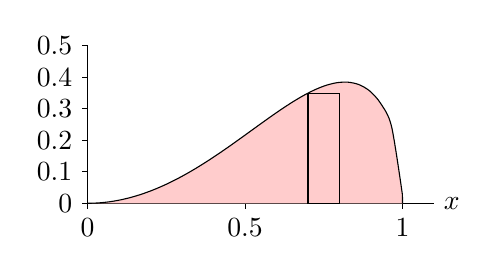
\begin{tikzpicture}[baseline=0,x=4cm,y=4cm,smooth]
\draw (0,0) -- (1.1,0) node [right] {$x$};
\draw (0,0) -- (0,0.5) ;
\foreach \x in {0,0.5,1} \draw (\x,0) -- (\x,-2pt) node[anchor=north] {$\x$};
\foreach \y in {0,0.1,0.2,0.3,0.4,0.5} \draw (0,\y) -- (-2pt,\y) node[anchor=east] {$\y$};
\draw[fill=red!20,domain=0:1,samples=30] plot (\x,{\x*\x*sqrt(1-\x*\x)}) -- (1,0);
\draw (0.7,0) rectangle (0.8,0.35); 
\end{tikzpicture}\hfill
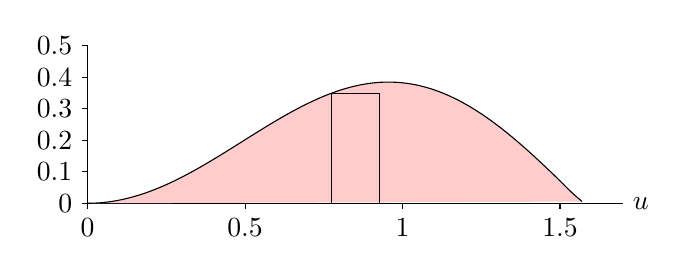
\begin{tikzpicture}[baseline=0,x=4cm,y=4cm,smooth]
\draw (0,0) -- (1.7,0) node [right] {$u$};
\draw (0,0) -- (0,0.5) ;
\foreach \x in {0,0.5,1,1.5} \draw (\x,0) -- (\x,-2pt) node[anchor=north] {$\x$};
\foreach \y in {0,0.1,0.2,0.3,0.4,0.5} \draw (0,\y) -- (-2pt,\y) node[anchor=east] {$\y$};
\draw[fill=red!20,domain=0:pi/2,samples=50] plot (\x,{sin(deg(\x))*sin(deg(\x))*sqrt(1-sin(deg(\x))*sin(deg(\x)))});
\draw (0.775,0) rectangle (0.927,0.35);
\end{tikzpicture}\hfill}
\caption{Single change of variable.}
\label{fig:onechangeofvariable}
\end{figure}

Let's examine the single variable case again, from a slightly
different perspective than we have previously used.
Suppose we start with the problem
\[\int_0^1 x^2\sqrt{1-x^2}\,dx;\]
this computes the area in the left graph of 
Figure~\ref{fig:onechangeofvariable}.
We use the substitution $x=\sin u$ to transform the function from 
$x^2\sqrt{1-x^2}$ to $\sin^2u\sqrt{1-\sin^2u}$, and we also convert
$dx$ to $\cos u\,du$. Finally, we convert the
limits 0 and 1 to 0 and $\pi/2$.
This transforms the integral:
\[\int_0^1 x^2\sqrt{1-x^2}\,dx=\int_0^{\pi/2}\sin^2u\sqrt{1-\sin^2u} \cos u\,du.\]
We want to notice that there are three different conversions: the
main function, the differential $dx$, and the interval of
integration. The function is converted to
$\sin^2u\sqrt{1-\sin^2u}$, shown in the right-hand graph of 
Figure~\ref{fig:onechangeofvariable}. It is evident that the two
curves pictured there have the same $y$-values in the same order, but
the horizontal scale has been changed. Even though the heights are the
same, the two integrals
\[\int_0^1 x^2\sqrt{1-x^2}\,dx\qquad\hbox{and}\qquad
\int_0^{\pi/2}\sin^2u\sqrt{1-\sin^2u}\,du\]
are not the same; clearly the right hand area is larger. One way to
understand the problem is to note that if both areas are approximated
using, say, ten subintervals, that the approximating rectangles on the
right are wider than their counterparts on the left, as indicated. In
the picture, the width of the rectangle on the left is $\Delta x=0.1$,
between $0.7$ and $0.8$.  The rectangle on the right is situated
between the corresponding values $\arcsin(0.7)$ and $\arcsin(0.8)$ so
that $\Delta u=\arcsin(0.8)-\arcsin(0.7)$. To
make the widths match, and the areas therefore the same, we can
multiply $\Delta u$ by a correction factor; in this case the
correction factor is approximately $\cos u=\cos(\arcsin(0.7))$, which
we compute when we convert $dx$ to $\cos u\,du$.

Now let's move to functions of two variables. Suppose we want to
convert an integral
\[\int_{x_0}^{x_1}\int_{y_0}^{y_1} f(x,y)\,dy\,dx\]
to use new variables $u$ and $v$. In the single variable case, there's
typically just one reason to want to change the variable: to make the
function ``nicer'' so that we can find an antiderivative. In the two
variable case, there is a second potential reason: the two-dimensional
region over which we need to integrate is somehow unpleasant, and we
want the region in terms of $u$ and $v$ to be nicer---to be a
rectangle, for example. Ideally, of course, the new function and the
new region will be no worse than the originals, and at least one of
them will be better; this doesn't always pan out.

As before, there are three parts to the conversion: the function
itself must be rewritten in terms of $u$ and $v$, $dy\,dx$ must be
converted to $du\,dv$, and the old region must be converted to the new
region. We will develop the necessary techniques by considering a
particular example, and we will use an example we already know how to
do by other means.

Consider 
\[\int_{-1}^1\int_0^{\sqrt{1-x^2}} \sqrt{x^2+y^2}\,dy\,dx.\]
The limits correspond to integrating over the top half of a circular
disk, and we recognize that the function will simplify in polar
coordinates, so we would normally convert to polar coordinates:
\[\int_{0}^\pi\int_0^1 \sqrt{r^2}\;r\,dr\,d\theta={\pi\over3}.\]
But let's instead approach this as a substitution problem, starting
with $x=r\cos\theta$, $y=r\sin\theta$. This pair of equations
describes a function from ``$r$-$\theta$ space'' to ``$x$-$y$ space'',
and because it involves familiar concepts, it is not too hard to
understand what it does. In Figure~\ref{fig:twodimensionaltransformation}
we have indicated geometrically a bit about how this
function behaves. The four dots labeled \emph{a}--\emph{d} in the $r$-$\theta$ plane
correspond to the three dots in the $x$-$y$ plane; dots \emph{a} and 
\emph{b} both go to the origin because $r=0$. The horizontal arrow in the
$r$-$\theta$ plane has $r=1$ everywhere and $\theta$ ranges from 0 to
$\pi$, so the corresponding points 
$x=r\cos\theta$, $y=r\sin\theta$ start at $(1,0)$ and follow the unit
circle counter-clockwise. Finally, the vertical arrow has
$\theta=\pi/4$ and $r$ ranges from 0 to 1, so it maps to the straight
arrow in the $x$-$y$ plane. Extrapolating from these few examples,
it's not hard to see that every vertical line in the $r$-$\theta$ plane
is transformed to a line through the origin in the $x$-$y$ plane, and
every horizontal line in the $r$-$\theta$ plane
is transformed to a circle with center at the origin in the $x$-$y$
plane. Since we are interested in integrating over the half-disk in
the $x$-$y$ plane, we will integrate over the rectangle
$[0,\pi]\times[0,1]$ in the $r$-$\theta$ plane, because we now see
that the points in this rectangle are sent precisely to the upper half
disk by $x=r\cos\theta$ and $y=r\sin\theta$.

\begin{figure}[H]
\centerline{
\vbox{\beginpicture
\normalgraphs
\setcoordinatesystem units <2truecm,2truecm>
\setplotarea x from 0 to 3.2, y from 0 to 1.1
\axis left ticks numbered from 0 to 1 by 1 /
\axis bottom  ticks withvalues {$\pi$} / at 3.14 / /
\put {$\theta$} [l] <3pt,0pt> at 3.2 0
\put {$r$} [b] <0pt,3pt> at 0 1.1
\arrow <5pt> [0.17, 0.5] from 0 1 to 3.14 1
\arrow <5pt> [0.17, 0.5] from 0.785 0 to 0.785 1
\multiput {$\bullet$} at 0 0 1.57 0 0 1 1.57 0.5 /
\put {$a$} [t] <0pt,-4pt> at 0 0
\put {$b$} [t] <0pt,-4pt> at 1.57 0
\put {$c$} [tl] <2pt,-2pt> at 0 1
\put {$d$} [tr] <-2pt,-2pt> at 1.57 0.5
\setcoordinatesystem units <2truecm,2truecm> point at -6 0
\setplotarea x from -1.1 to 1.1, y from 0 to 1.1
\axis left shiftedto x=0 /
\axis bottom  ticks numbered from -1 to 1 by 1 /
\put {$x$} [l] <3pt,0pt> at 1.1 0
\put {$y$} [b] <0pt,3pt> at 0 1.1
\multiput {$\bullet$} at 0 0 1 0 0 0.5 /
\put {$a,b$} [br] <-2pt,2pt> at 0 0
\put {$c$} [br] <-2pt,2pt> at 1 0
\put {$d$} [br] <-2pt,2pt> at 0 0.5
\arrow <5pt> [0.17, 0.5] from 0 0 to 0.707 0.707
\circulararc 180 degrees from 1 0 center at 0 0
\multiput {\beginpicture % 
\setcoordinatesystem units <0.4truein,0.4truein> point at 0 0
\startrotation by 0 -1 about 0 0 %
\plot -.1 .05 0 0 -.1 -.05 / \endpicture} at -1 0 /
\endpicture}}
\caption{Double change of variable.}
\label{fig:twodimensionaltransformation}
\end{figure}

At this point we are two-thirds done with the task: we know the
$r$-$\theta$ limits of integration, and we can easily convert the
function to the new variables:
\begin{equation}\label{eq:transformedfunction}
\sqrt{x^2+y^2}=\sqrt{r^2\cos^2\theta+r^2\sin^2\theta}=r\sqrt{\cos^2\theta+\sin^2\theta} = r.
\end{equation}
The final, and most difficult, task is to figure out what replaces
$dx\,dy$. (Of course, we actually know the answer, because we are in
effect converting to polar coordinates. What we really want is a
series of steps that gets to that right answer but that will also work
for other substitutions that are not so familiar.)

Let's take a step back and remember how integration arises from
approximation. When we approximate the integral in the $x$-$y$ plane,
we are computing the volumes of tall thin boxes, in this case boxes
that are $\Delta x\times \Delta y\times \sqrt{x^2+y^2}$. We are aiming
to come up with an integral in the $r$-$\theta$ plane that looks like
this:
\begin{equation}\label{eq:targetintegral}
\int_0^\pi\int_0^1 r (?) \,dr\,d\theta.
\end{equation}
What we're missing is exactly the right quantity to replace the ``?''
so that we get the correct answer. Of course, this integral is also
the result of an approximation, in which we add up volumes of boxes
that are $\Delta r\times\Delta \theta\times\hbox{height}$; the problem
is that the height that will give us the correct answer is not simply
$r$. Or put another way, we can think of the correct height as $r$,
but the area of the base $\Delta r\Delta\theta$ as being wrong. The
height $r$ comes from Equation~\ref{eq:transformedfunction}, which
is to say, it is precisely the same as the corresponding height in the
$x$-$y$ version of the integral. The problem is that the area of the
base $\Delta x\times \Delta y$ is not the same as the area of the base
$\Delta r\times\Delta\theta$. We can think of the ``?'' in the integral as a
correction factor that is needed so that
$?\,dr\,d\theta$ = $dx\,dy$.

So let's think about what that little base $\Delta
r\times\Delta\theta$ corresponds to. We know that each bit of
horizontal line in the $r$-$\theta$ plane corresponds to a bit of
circular arc in the $x$-$y$ plane, and each bit of vertical line
in the $r$-$\theta$ plane corresponds to a bit of
``radial line'' in the $x$-$y$ plane. In
Figure~\ref{fig:correspondingareas} we show a typical rectangle in
the $r$-$\theta$ plane and its corresponding area in the $x$-$y$ plane.

\begin{figure}[H]
\centerline{
\vbox{\beginpicture
\normalgraphs
\setcoordinatesystem units <2truecm,2truecm>
\setplotarea x from 0 to 3.2, y from 0 to 1.1
\axis left ticks numbered from 0 to 1 by 1 /
\axis bottom  ticks withvalues {$\pi$} / at 3.14 / /
\put {$\theta$} [l] <3pt,0pt> at 3.2 0
\put {$r$} [b] <0pt,3pt> at 0 1.1
\put {$\Delta r$} [r] <-3pt,0pt> at 2.094 0.625
\put {$\Delta\theta$} [t] <0pt,-3pt> at 2.356 0.5
\plot 2.094 0.5 2.094 0.75 2.618 0.75 2.618 0.5 2.094 0.5 /
\setcoordinatesystem units <2truecm,2truecm> point at -6 0
\setplotarea x from -1.1 to 1.1, y from 0 to 1.1
\axis left shiftedto x=0 /
\axis bottom  ticks numbered from -1 to 1 by 1 /
\put {$x$} [l] <3pt,0pt> at 1.1 0
\put {$y$} [b] <0pt,3pt> at 0 1.1
%\put {$\Delta r$} [tr] <-2pt,-2pt> at -0.54 0.31
%\put {$r\Delta\theta$} [br] <-2pt,2pt> at -0.53 0.53
\circulararc 30 degrees from -0.25 0.433 center at 0 0
\circulararc 30 degrees from -0.375 0.65 center at 0 0
\plot -0.25 0.433 -0.375 0.65 /
\plot -0.433 0.25 -0.65 0.375 /
\endpicture}}
\caption{Corresponding areas.}
\label{fig:correspondingareas}
\end{figure}

In this case, the region in the $x$-$y$ plane is approximately a
rectangle with dimensions $\Delta r\times r\Delta\theta$, but in
general the corner angles will not be right angles, so the region will
typically be (almost) a parallelogram. We need to compute the area of
this parallelogram. We know
a neat way to do this: compute the length of a certain cross product.
If we can determine an appropriate two vectors we'll be nearly done.

Fortunately, we've really done this before. The sides of the region in
the $x$-$y$ plane are formed by temporarily fixing either $r$ or
$\theta$ and letting the other variable range over a small interval.
In Figure~\ref{fig:correspondingareas}, for example, the upper right
edge of the region is formed by fixing $\theta=2\pi/3$ and letting $r$
run from $0.5$ to $0.75$. In other words, we have a vector function
$\vect{v}(r)=\langle r\cos\theta_0, r\sin\theta_0, 0\rangle$, and we
are interested in a restricted set of values for $r$. A vector tangent
to this path is given by the derivative $\vect{v}'(r)=\langle
\cos\theta_0, \sin\theta_0, 0\rangle$, and a small tangent vector,
with length approximately equal to the side of the region, is $\langle
\cos\theta_0, \sin\theta_0, 0\rangle\,dr$. Likewise, if we fix
$r=r_0=0.5$, we get the vector function $\vect{w}(\theta)=\langle
r_0\cos\theta, r_0\sin\theta, 0\rangle$ with derivative $\vect{w}(\theta)=\langle -r_0\sin\theta, r_0\cos\theta, 0\rangle$ and a
small tangent vector $\langle -r_0\sin\theta_0, r_0\cos\theta_0,
0\rangle\,d\theta$ when $\theta=\theta_0$ (at the corner we're
focusing on). These vectors are shown in 
Figure~\ref{fig:smallapproximatingparallelogram}, with the actual
region outlined by a dotted boundary. Of course, since both $\Delta r$
and $\Delta\theta$ are quite large, the parallelogram is not a
particularly good approximation to the true area.

\begin{figure}[H]
\centerline{
\vbox{\beginpicture
\normalgraphs
\setcoordinatesystem units <3truecm,3truecm> 
\setplotarea x from -1.1 to 1.1, y from 0 to 1.1
\axis left shiftedto x=0 /
\axis bottom  ticks numbered from -1 to 1 by 1 /
\put {$x$} [l] <3pt,0pt> at 1.1 0
\put {$y$} [b] <0pt,3pt> at 0 1.1
%\put {$\Delta r$} [tr] <-2pt,-2pt> at -0.54 0.31
%\put {$r\Delta\theta$} [br] <-2pt,2pt> at -0.53 0.53
\arrow <5pt> [0.17, 0.5] from  -0.25 0.433  to  -0.375 0.65
\arrow <5pt> [0.17, 0.5] from -0.25 0.433 to -0.477  0.302
\setdashes
\plot -0.477  0.302 -0.602 0.519 -0.375 0.65 /
\findlength{\circulararc 30 degrees from -0.25 0.433 center at 0 0 }
\setdotsnear <2pt> for <\totalarclength>
\circulararc 30 degrees from -0.25 0.433 center at 0 0
\findlength{\circulararc 30 degrees from -0.375 0.65 center at 0 0 }
\setdotsnear <2pt> for <\totalarclength>
\circulararc 30 degrees from -0.375 0.65 center at 0 0
\setlinear
\plot -0.433 0.25 -0.65 0.375 /
\endpicture}}
\caption{The approximating parallelogram.}
\label{fig:smallapproximatingparallelogram}
\end{figure}

The area of this parallelogram is the length of the cross product:
\begin{align*}
\langle -r_0\sin\theta_0, r_0\cos\theta_0, 0\rangle\,d\theta\times\langle\cos\theta_0, \sin\theta_0, 0\rangle\,dr
&= \left|\begin{matrix}	\vect{i}			&	\vect{j}		&	\vect{k}	\\
						-r_0\sin\theta_0	&	r_0\cos\theta_0	&	0			\\
						\cos\theta_0		&	\sin\theta_0	&	0
		 \end{matrix}\right|\,d\theta\,dr	\\
&=\langle 0,0,-r_0\sin^2\theta_0-r_0\cos^2\theta_0\rangle\,d\theta\,dr	\\
&=\langle 0,0,-r_0\rangle\,d\theta\,dr.
\end{align*}
The length of this vector is $r_0\,dr\,d\theta$. So in general, for
any values of $r$ and $\theta$, the area in the $x$-$y$ plane
corresponding to a small rectangle anchored at $(\theta,r)$ in the
$r$-$\theta$ plane is approximately $r\,dr\,d\theta$. In other words, ``$r$''
replaces the ``?'' in Equation~\ref{eq:targetintegral}.

In general, a substitution will start with equations $x=f(u,v)$ and
$y=g(u,v)$. Again, it will be straightforward to convert the function
being integrated. Converting the limits will require, as above, an
understanding of just how the functions $f$ and $g$ transform the
$u$-$v$ plane into the $x$-$y$ plane. Finally, the small vectors we
need to approximate an area will be
$\langle f_u,g_u,0\rangle\,du$ and $\langle f_v,g_v,0\rangle\,dv$.
The cross product of these is $\langle
0,0,f_ug_v-g_uf_v\rangle\,du\,dv$ with length 
$|f_ug_v-g_uf_v|\,du\,dv$. The quantity $|f_ug_v-g_uf_v|$ is usually
denoted
$$\left|{\partial(x,y)\over\partial(u,v)}\right|=|f_ug_v-g_uf_v|$$
and called the \dfont{Jacobian}\index{Jacobian}.
Note that this is the absolute value of the two by two determinant
\[\left|\begin{matrix}	f_u	&	g_u	\\
						f_v	&	g_v
		\end{matrix}\right|,\]
which may be easier to remember. (Confusingly, the matrix, the
determinant of the matrix, and the absolute value of the determinant
are all called the Jacobian by various authors.)

Because there are two things to worry about, namely, the form of the
function and the region of integration, transformations in two (or
more) variables are quite tricky to discover.

\begin{example}{Integral of an Ellipse}{changeofvariables}
Integrate $x^2-xy+y^2$ over the region $x^2-xy+y^2\le 2$.
\end{example}
\begin{solution}
The equation $x^2-xy+y^2= 2$ describes an ellipse as in
Figure~\ref{fig:skewedellipse}; the region of integration is the
interior of the ellipse. We will use the transformation 
$x=\sqrt2 u-\sqrt{2/3}v$, $y=\sqrt2 u+\sqrt{2/3}v$.
Substituting into the function itself we get
\[x^2-xy+y^2=2u^2+2v^2.\]
The boundary of the ellipse is $x^2-xy+y^2=2$, so the boundary of
the corresponding region in the $u$-$v$ plane is $2u^2+2v^2=2$
or $u^2+v^2=1$, the unit circle, so this substitution makes the region
of integration simpler. 

Next, we compute the Jacobian, using $f=\sqrt2 u-\sqrt{2/3}v$ and 
$g=\sqrt2 u+\sqrt{2/3}v$:
\[f_ug_v-g_uf_v=\sqrt2\sqrt{2/3}+\sqrt2\sqrt{2/3}={4\over\sqrt3}.\]
Hence the new integral is 
\[\iint_R (2u^2+2v^2){4\over\sqrt3}\,du\,dv,\]
where $R$ is the interior of the unit circle.
This is still not an easy integral, but it is easily transformed to
polar coordinates, and then easily integrated.
\end{solution}

\begin{figure}[H]
\centerline{
\vbox{\beginpicture
\normalgraphs
\setcoordinatesystem units <1.2truecm,1.2truecm> 
\setplotarea x from -2 to 2, y from -2 to 2
\axis left shiftedto x=0 /
\axis bottom shiftedto y=0  /
\put {$x$} [l] <3pt,0pt> at 2 0
\put {$y$} [b] <0pt,3pt> at 0 2
\plot -1.630 -0.729 -1.548 -0.325 -1.467 -0.112 -1.386 0.056 -1.304 0.199 
-1.222 0.326 -1.141 0.441 -1.060 0.546 -0.978 0.644 -0.896 0.734 
-0.815 0.818 -0.734 0.897 -0.652 0.971 -0.570 1.040 -0.489 1.105 
-0.408 1.166 -0.326 1.223 -0.244 1.276 -0.163 1.326 -0.082 1.372 
0.000 1.414 0.082 1.453 0.163 1.489 0.244 1.521 0.326 1.549 
0.408 1.573 0.489 1.594 0.570 1.610 0.652 1.623 0.734 1.630 
0.815 1.633 0.896 1.630 0.978 1.622 1.060 1.606 1.141 1.582 
1.222 1.549 1.304 1.503 1.386 1.441 1.467 1.355 1.548 1.223 
1.630 0.901 /
\plot -1.630 -0.901 -1.548 -1.223 -1.467 -1.355 -1.386 -1.441 -1.304 -1.503 
-1.222 -1.549 -1.141 -1.582 -1.060 -1.606 -0.978 -1.622 -0.896 -1.630 
-0.815 -1.633 -0.734 -1.630 -0.652 -1.623 -0.570 -1.610 -0.489 -1.594 
-0.408 -1.573 -0.326 -1.549 -0.244 -1.521 -0.163 -1.489 -0.082 -1.453 
0.000 -1.414 0.082 -1.372 0.163 -1.326 0.244 -1.276 0.326 -1.223 
0.408 -1.166 0.489 -1.105 0.570 -1.040 0.652 -0.971 0.734 -0.897 
0.815 -0.818 0.896 -0.734 0.978 -0.644 1.060 -0.546 1.141 -0.441 
1.222 -0.326 1.304 -0.199 1.386 -0.056 1.467 0.112 1.548 0.325 
1.630 0.729 /
\plot 1.63 0.729 1.633 0.8164965809 1.63 0.901 /
\plot -1.63 -0.729 -1.633 -0.8164965809 -1.63 -0.901 /
\endpicture}}
\caption{$x^2-xy+y^2=2$}
\label{fig:skewedellipse}
\end{figure}

There is a similar change of variables formula for triple integrals,
though it is a bit more difficult to derive.
Suppose we use three substitution functions, $x=f(u,v,w)$,
$y=g(u,v,w)$, and $z=h(u,v,w)$.  The Jacobian determinant is now
\[
  {\partial(x,y,z)\over\partial(u,v,w)} =  
  \left|\begin{matrix}	f_u	&	g_u	&	h_u	\\
  						f_v	&	g_v	&	h_v	\\
  						f_w	&	g_w	&	h_w
  		\end{matrix}\right|.
\]
Then the integral is transformed in a similar fashion:
\[
  \iiint_R F(x,y,z) \, dV = 
  \iiint_S F(f(u,v,w),g(u,v,w),h(u,v,w)) 
  \left|{\partial(x,y,z)\over\partial(u,v,w)}\right| \,du\,dv\,dw,
\]
where of course the region $S$ in $uvw$ space corresponds to the
region $R$ in $xyz$ space.


%%%%%%%%%%%%%%%%%%%%%%%%%%%%%%%%%%%%%%%%%%%%
\Opensolutionfile{solutions}[ex]
\section*{Exercises for \ref{sec:ChangeofVariables}}

\begin{enumialphparenastyle}

\begin{ex}
Complete Example~\ref{exa:changeofvariables} by
converting to polar coordinates and evaluating the integral.
\begin{sol}
$\ds 4\pi\sqrt3/3$
\end{sol}
\end{ex}

\begin{ex}
Evaluate $\ds\iint xy\,dx\,dy$ over the square
with corners $(0,0)$, $(1,1)$, $(2,0)$, and $(1,-1)$ in two ways:
directly, and using $x=(u+v)/2$, $y=(u-v)/2$.
\begin{sol}
$0$
\end{sol}
\end{ex}

\begin{ex}
Evaluate $\ds\iint x^2+y^2\,dx\,dy$ over the square
with corners $(-1,0)$, $(0,1)$, $(1,0)$, and $(0,-1)$ in two ways:
directly, and using $x=(u+v)/2$, $y=(u-v)/2$.
\begin{sol}
$2/3$
\end{sol}
\end{ex}

\begin{ex}
Evaluate $\ds\iint (x+y)e^{x-y}\,dx\,dy$ over the triangle
with corners $(0,0)$, $(-1,1)$, and $(1,1)$ in two ways:
directly, and using $x=(u+v)/2$, $y=(u-v)/2$.
\begin{sol}
$\ds {e^2-1\over 2e^2}$
\end{sol}
\end{ex}

\begin{ex}
Evaluate $\ds\iint y(x-y)\,dx\,dy$ over the parallelogram
with corners $(0,0)$, $(3,3)$, $(7,3)$, and $(4,0)$ in two ways:
directly, and using $x=u+v$, $y=u$.
\begin{sol}
$36$
\end{sol}
\end{ex}

\begin{ex}
Evaluate $\ds\iint \sqrt{x^2+y^2}\,dx\,dy$ over the
triangle with corners $(0,0)$, $(4,4)$, and $(4,0)$ using $x=u$, $y=uv$.
\begin{sol}
$32(\sqrt2+\ln(1+\sqrt2))/3$
\end{sol}
\end{ex}

\begin{ex}
Evaluate $\ds\iint y\sin(xy)\,dx\,dy$ over the
region bounded by $xy=1$, $xy=4$, $y=1$, and $y=4$ using
$x=u/v$, $y=v$.
\begin{sol}
$3\cos(1)-3\cos(4)$
\end{sol}
\end{ex}

\begin{ex}
Evaluate $\ds\iint \sin(9x^2 + 4y^2)\,dA,$ over the region
 in the first quadrant bounded by the ellipse $9x^2+4y^2 = 1$.
\begin{sol}
$\pi(1-\cos(1))/24$
\end{sol}
\end{ex}

\begin{ex}
Compute the Jacobian for the substitutions 
$x=\rho\sin\phi\cos\theta$, $y=\rho\sin\phi\sin\theta$, 
$z=\rho\cos\phi$.
\end{ex}

\begin{ex}
Evaluate $\ds\iiint_E\,dV$ where $E$ is the solid
enclosed by the ellipsoid
$${x^2\over a^2} + {y^2\over b^2} + {z^2\over c^2} = 1,$$ 
using the transformation $x=au$, $y=bv$, and $z=cw$.
\begin{sol}
$(4/3)\pi abc$
\end{sol}
\end{ex}

\end{enumialphparenastyle}
